\documentclass[11pt, letterpaper]{report}
\input{../../homework.tex}
\usepackage{titlepageBU}
\title{Honors Differential Equations}
\date{11/20/24}
\courseID{MA 231}
\professor{Dr. Wayne}
\courseSection{A1}
\DeclareMathOperator{\Tr}{Tr}
\graphicspath{{../figures}}
\begin{document}
\makeproblem
\section*{Section 5.1 Problem 2}
The jacobian for systems 1, 2, and 3, are
 \[
	\mathbf{J}_1(\mathbf{x})=\begin{pmatrix}
		3\cos x&1\\
		4&-\sin y
	\end{pmatrix} ,\quad \mathbf{J}_2(\mathbf{x})=\begin{pmatrix}
		-3\cos x&1\\
		4&-\sin y
	\end{pmatrix} ,\quad \mathbf{J}_3(\mathbf{x})=\begin{pmatrix}
		-3\cos x&1\\
		4&-3\sin y
	\end{pmatrix} 
.\]
Evaluating at $\mathbf{0}$, we have
\[
	\mathbf{J}_1(\mathbf{0})=\begin{pmatrix}
		3&1\\
		4&0
		\end{pmatrix} ,\qquad \mathbf{J}_2(\mathbf{0})=\begin{pmatrix}
		-3&1\\
		4&0
	\end{pmatrix} ,\qquad \mathbf{J}_3(\mathbf{0})=\begin{pmatrix}
		-3&1\\
		4&0
	\end{pmatrix} 
.\]
Notice that $\mathbf{J}_2(\mathbf{0})=\mathbf{J}_3(\mathbf{0})$, so they will have the same behavior at $\mathbf{0}$. Moreover, $\Tr \mathbf{J}_1=3$ and $\Tr \mathbf{J}_2=-3$, so system 1 will have different behavior.
\section*{Section 5.1 Problem 3}
The jacbobian at $\mathbf{0}$ is
\[
	\mathbf{J}(\mathbf{0})=\begin{pmatrix}
		-2&1\\
		0&-1
	\end{pmatrix}
.\]
We then obtain the eigenvalues
\[
	\lambda ^2+3\lambda +2=0\implies \lambda \in \left\{ -2,-1 \right\} 
.\]
So $\mathbf{0}$ a sink. Eigenvectors are $(1,0)$ and $(1,1)$. I drew a very horrible very rough picture on a whiteboard of the behavior near $\mathbf{0}$. The figures aren't lining up nicely so the image will be first one on the next page.
\begin{figure}[ht]
	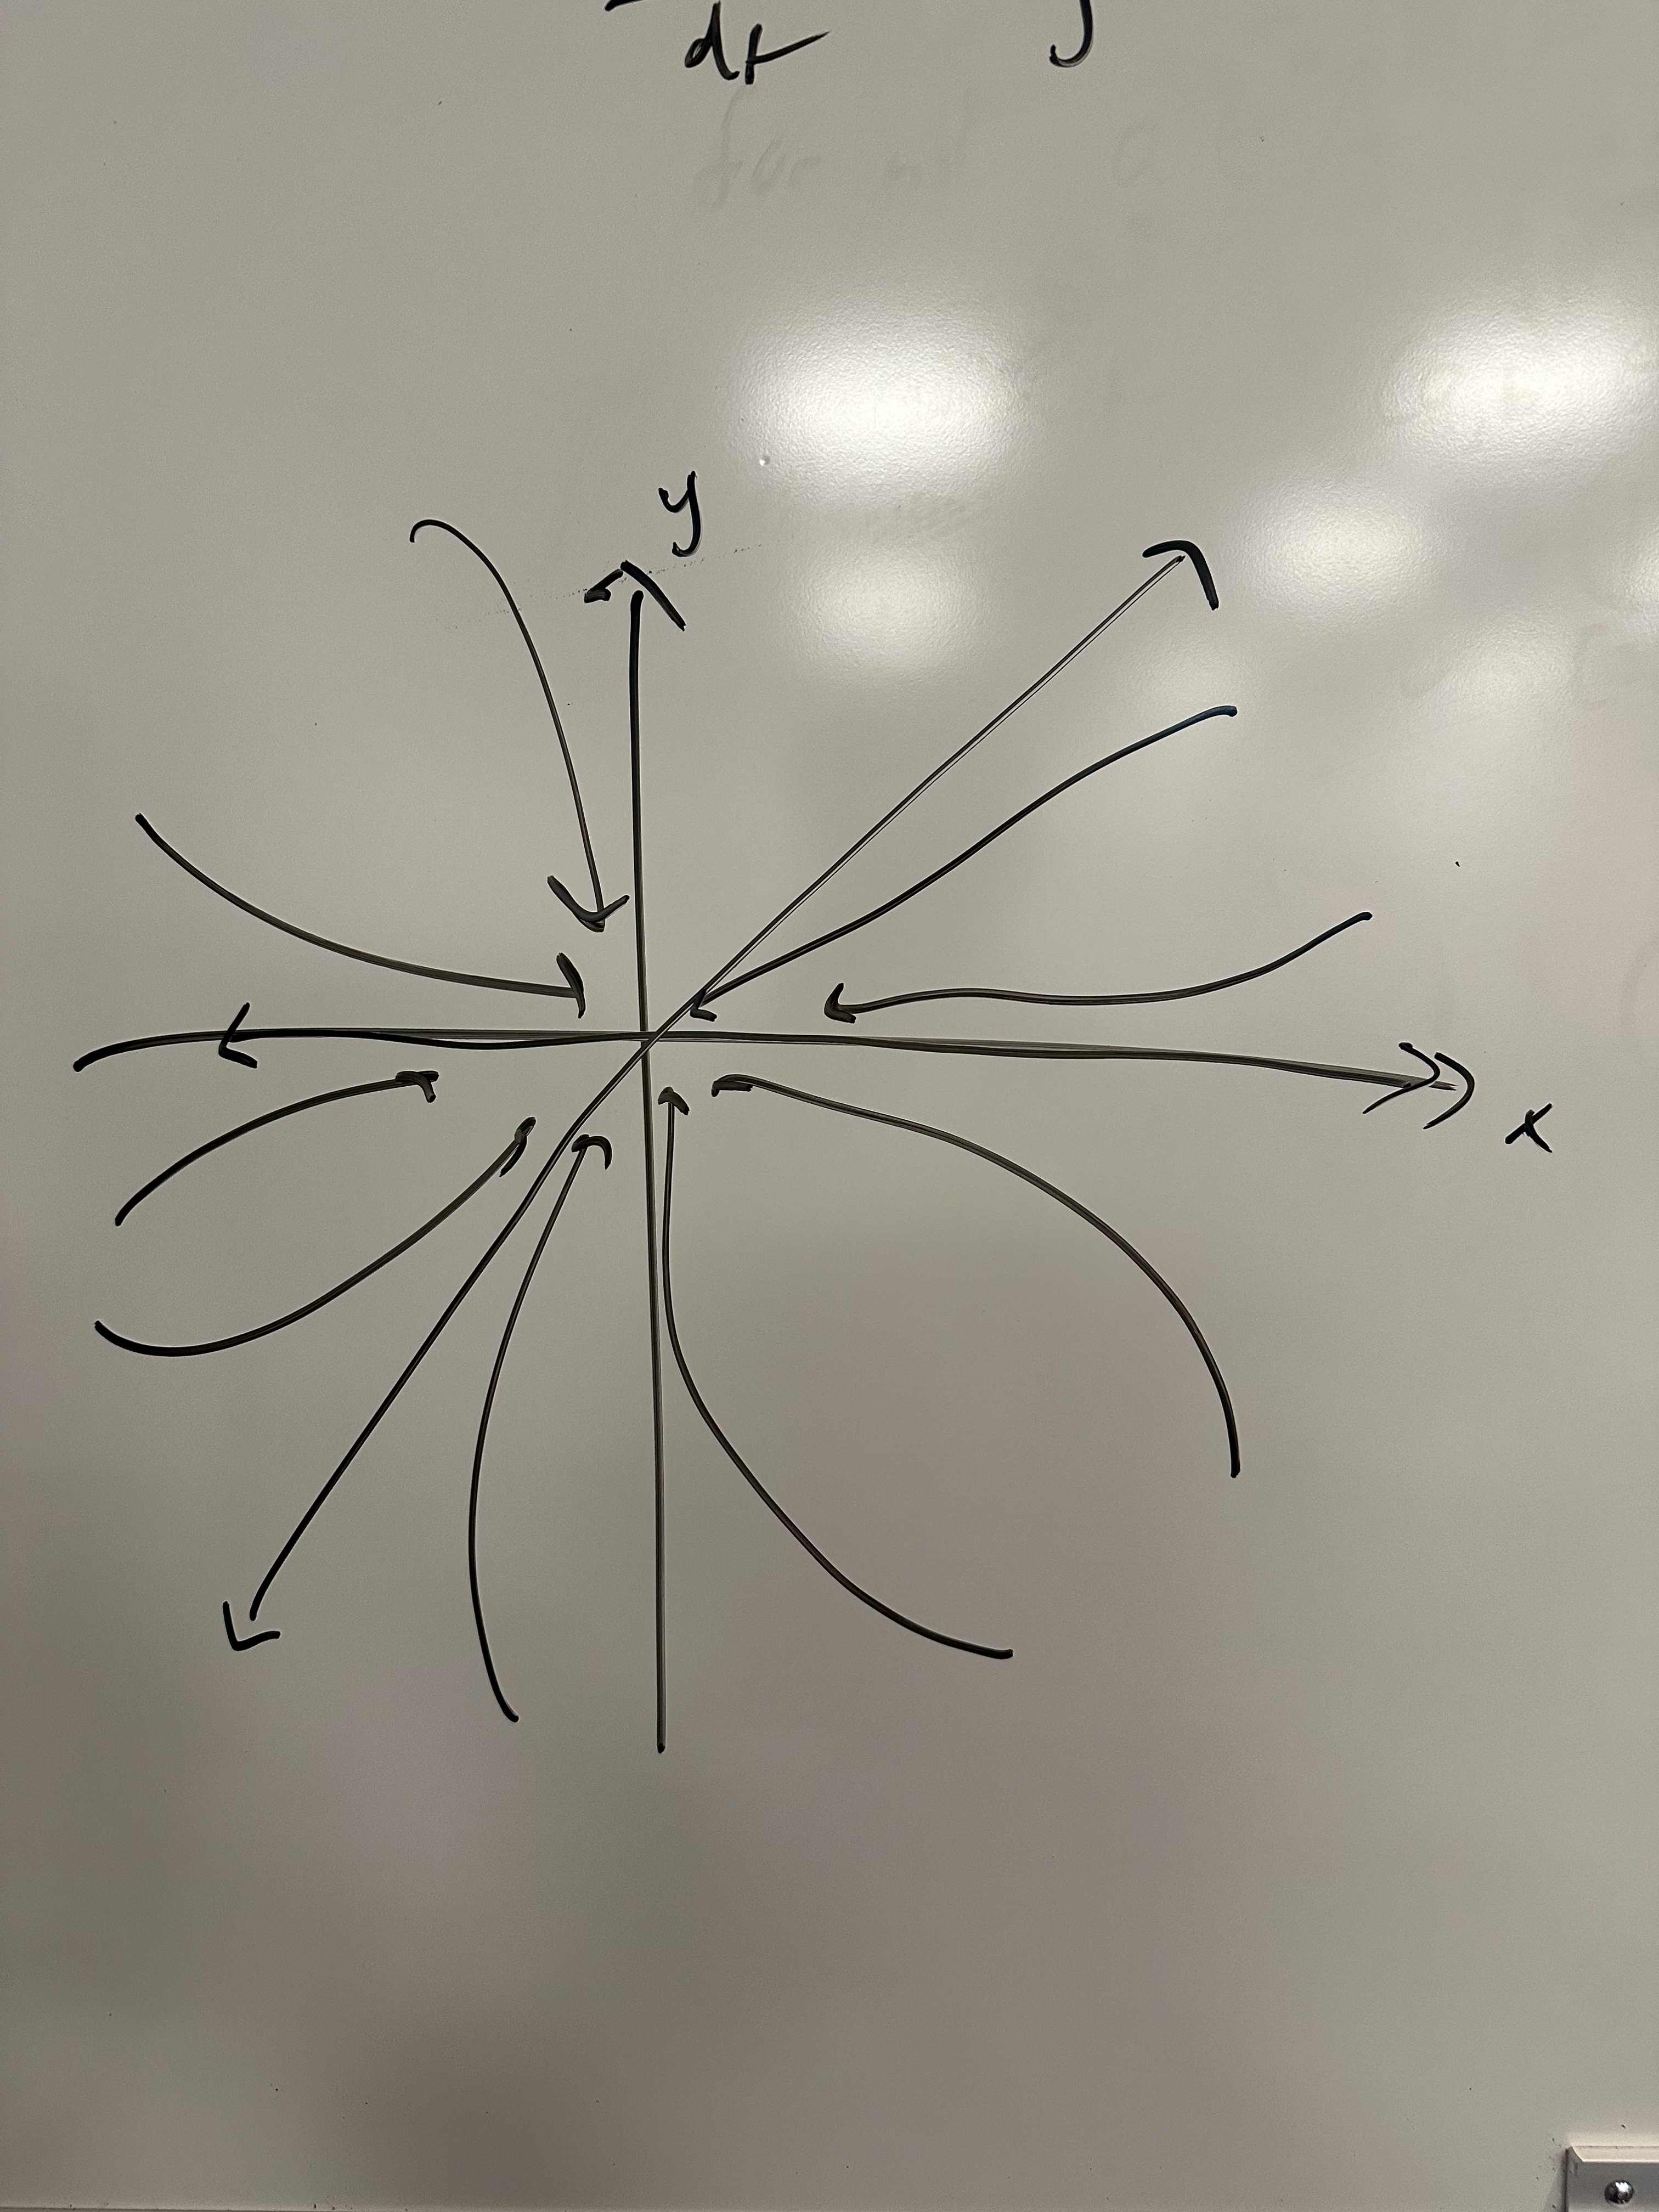
\includegraphics[scale=0.05]{1.png}
	\centering
	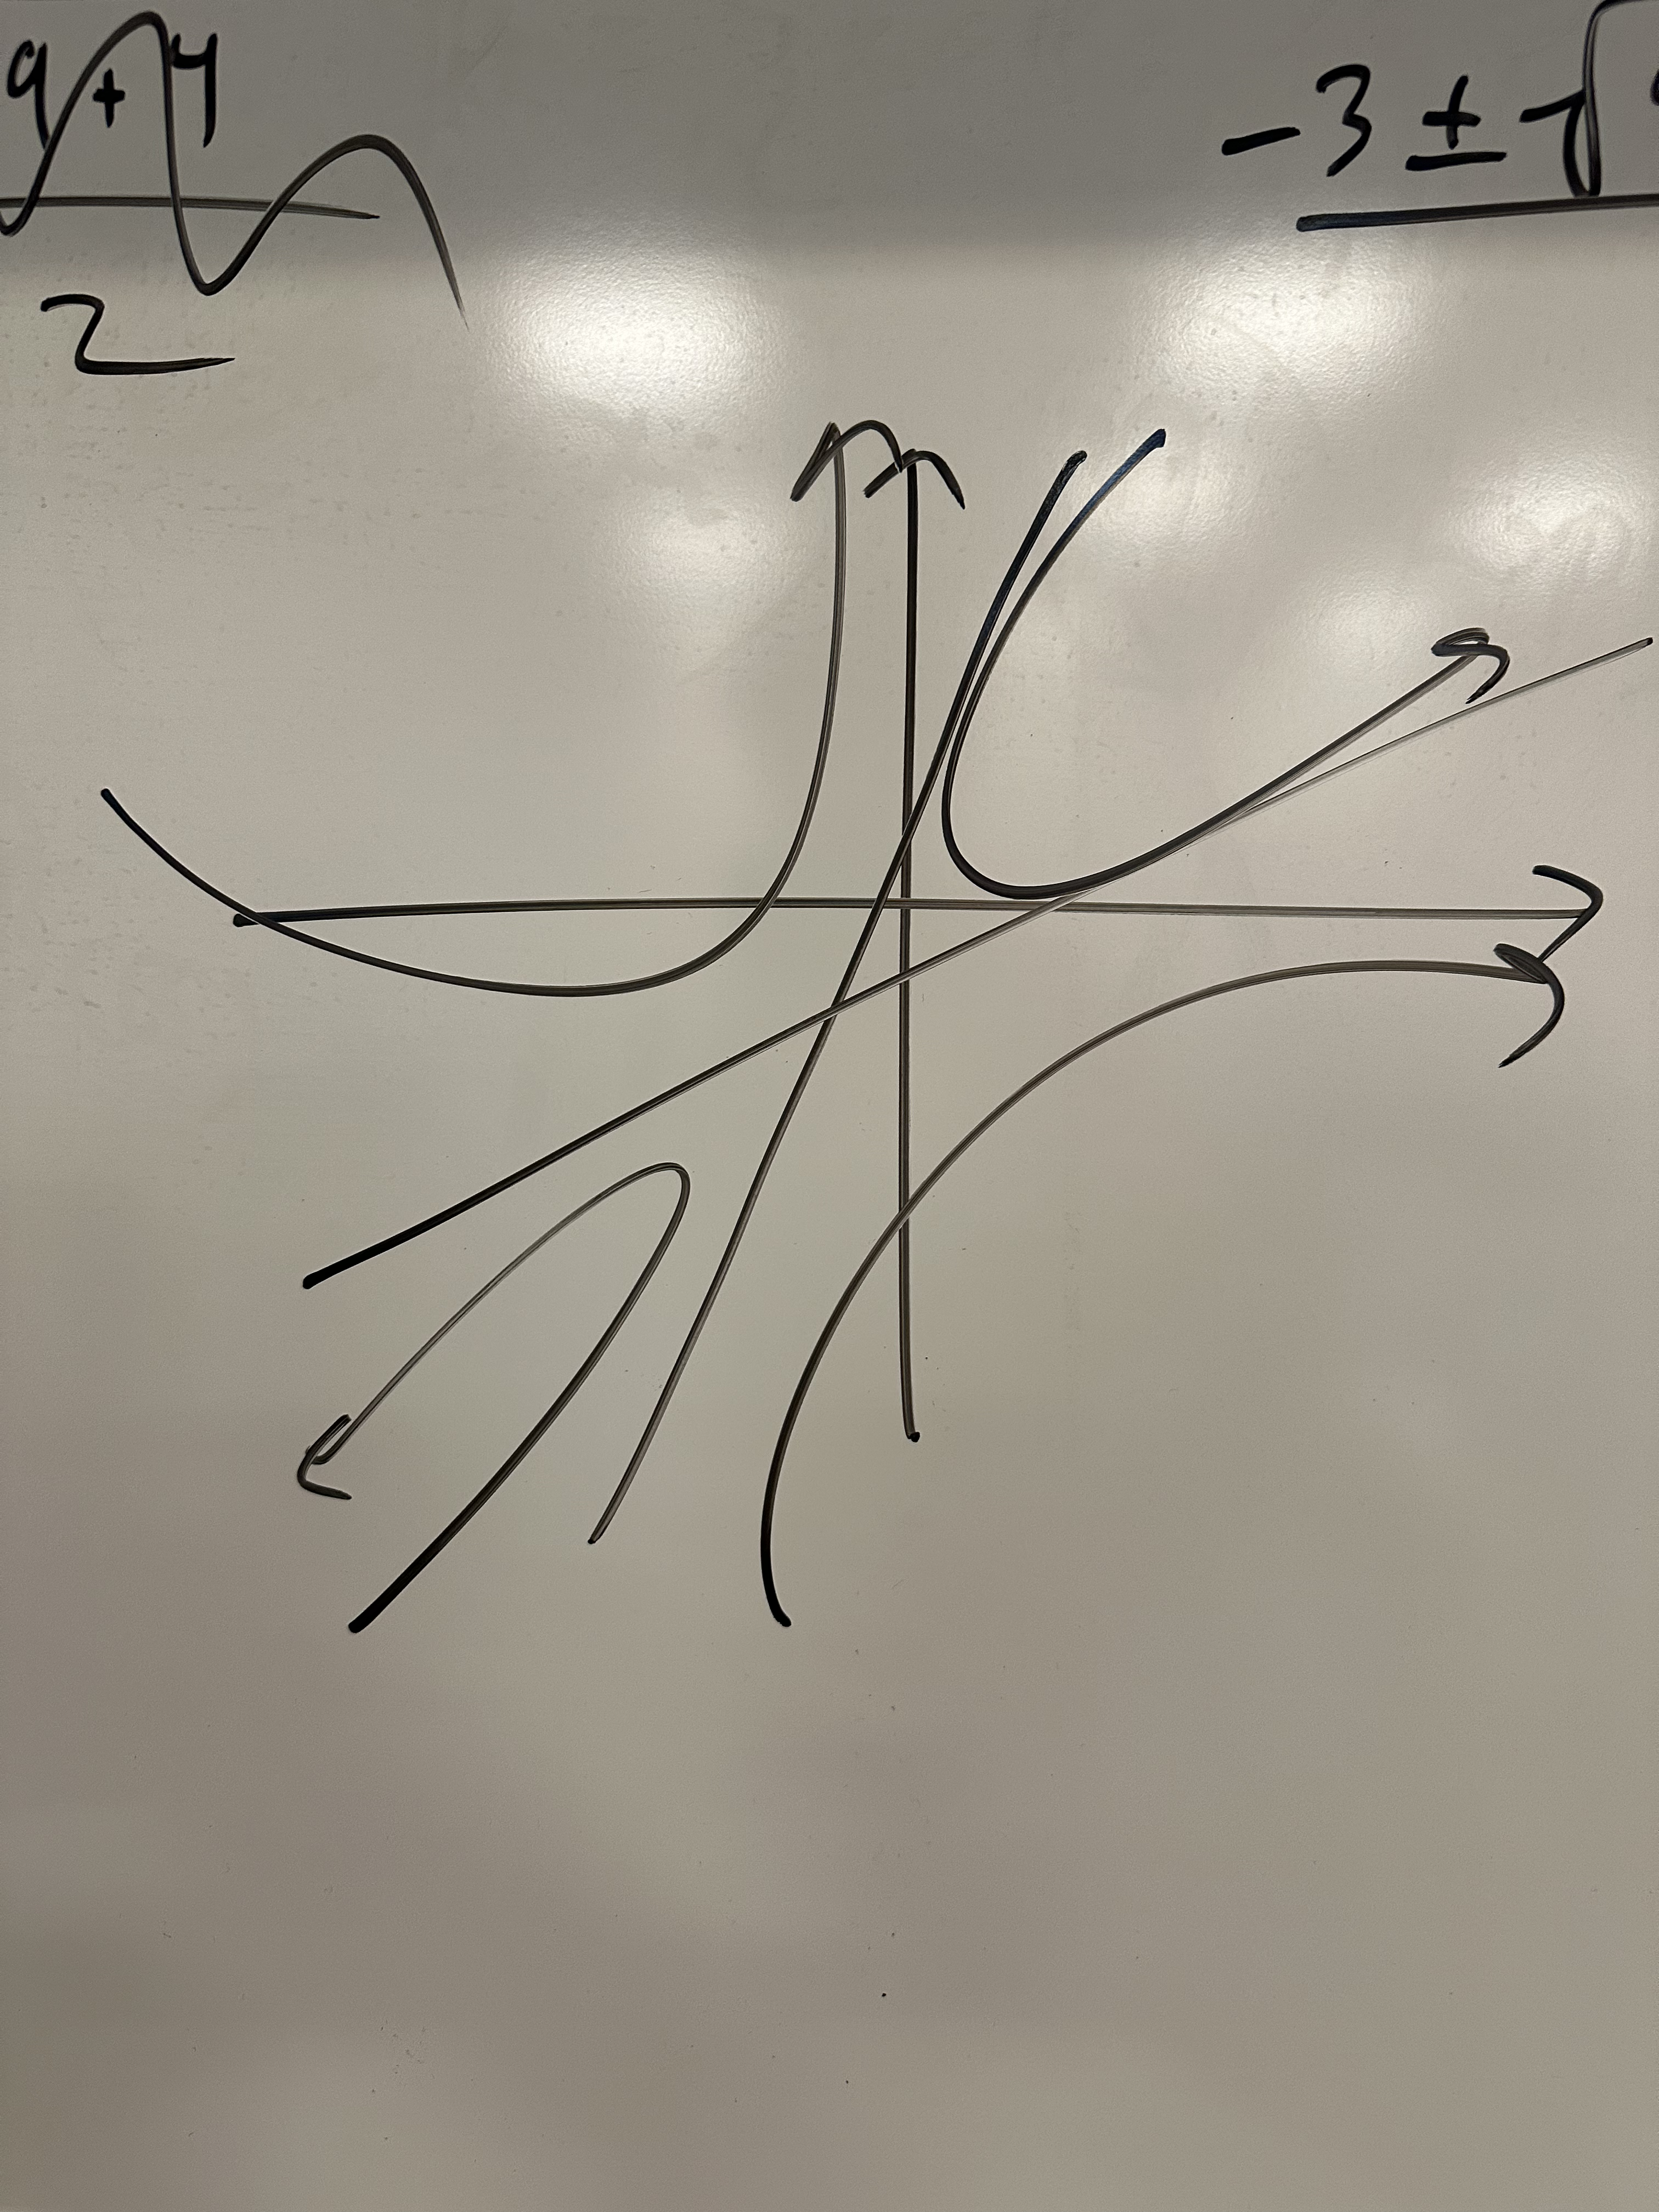
\includegraphics[scale=0.05]{IMG_2999.png}
	\centering
\end{figure}

Now the same process for $(2,4)$.
\[
	\mathbf{J}(2,4)=\begin{pmatrix}
		-2&1\\
		4&-1
	\end{pmatrix} 
.\]
\[
	\lambda ^2-3\lambda -2=0\implies \lambda = \frac{-3\pm \sqrt{17} }{2}
.\]
One positive, one negative, so $(2,4)$ is a saddle. The image will be the second image on the next page.
\newpage

\section*{Section 5.2 Problem 2}
First we solve for the nullclines. Letting $\frac{\mathrm{d}x}{\mathrm{d}t} =0$, we have $y=2-x$ and $(0,0)$ as the only solutions. Call the former an $x$-nullcline. Now letting $\frac{\mathrm{d}y}{\mathrm{d}t} =0$, we have $y=\left| x \right| $. Call this line a $y$-nullcline. They intersect at the point $(1,1)$, so this point is an equilibrium point.

Now consider the value of $\frac{\mathrm{d}y}{\mathrm{d}t} $ on the $x$-nullcline. We have
\[
	\frac{\mathrm{d}y}{\mathrm{d}t} =2-x-\left| x \right| =
	\begin{cases}
		2\left( 1-x \right) ,&x\geq 0\\
		2,&x<0
	\end{cases}
.\]
Notice that $\frac{\mathrm{d}y}{\mathrm{d}t} >0$ for all $x<1$, and $\frac{\mathrm{d}y}{\mathrm{d}t} <0$ for all $x>1$. Similarly, consider $\frac{\mathrm{d}x}{\mathrm{d}t} $ on the $y$-nullcline. We have
\[
	\frac{\mathrm{d}x}{\mathrm{d}t} =2-x-\left| x \right| =
	\begin{cases}
		2(1-x),&x\geq 0\\
		2,&x<0
	\end{cases}
.\]
This is the same behavior, less than 0 for $x>1$ and greater than 0 for $x<1$. Plotting the vector field, we have the following figure.
\begin{figure}[ht]
	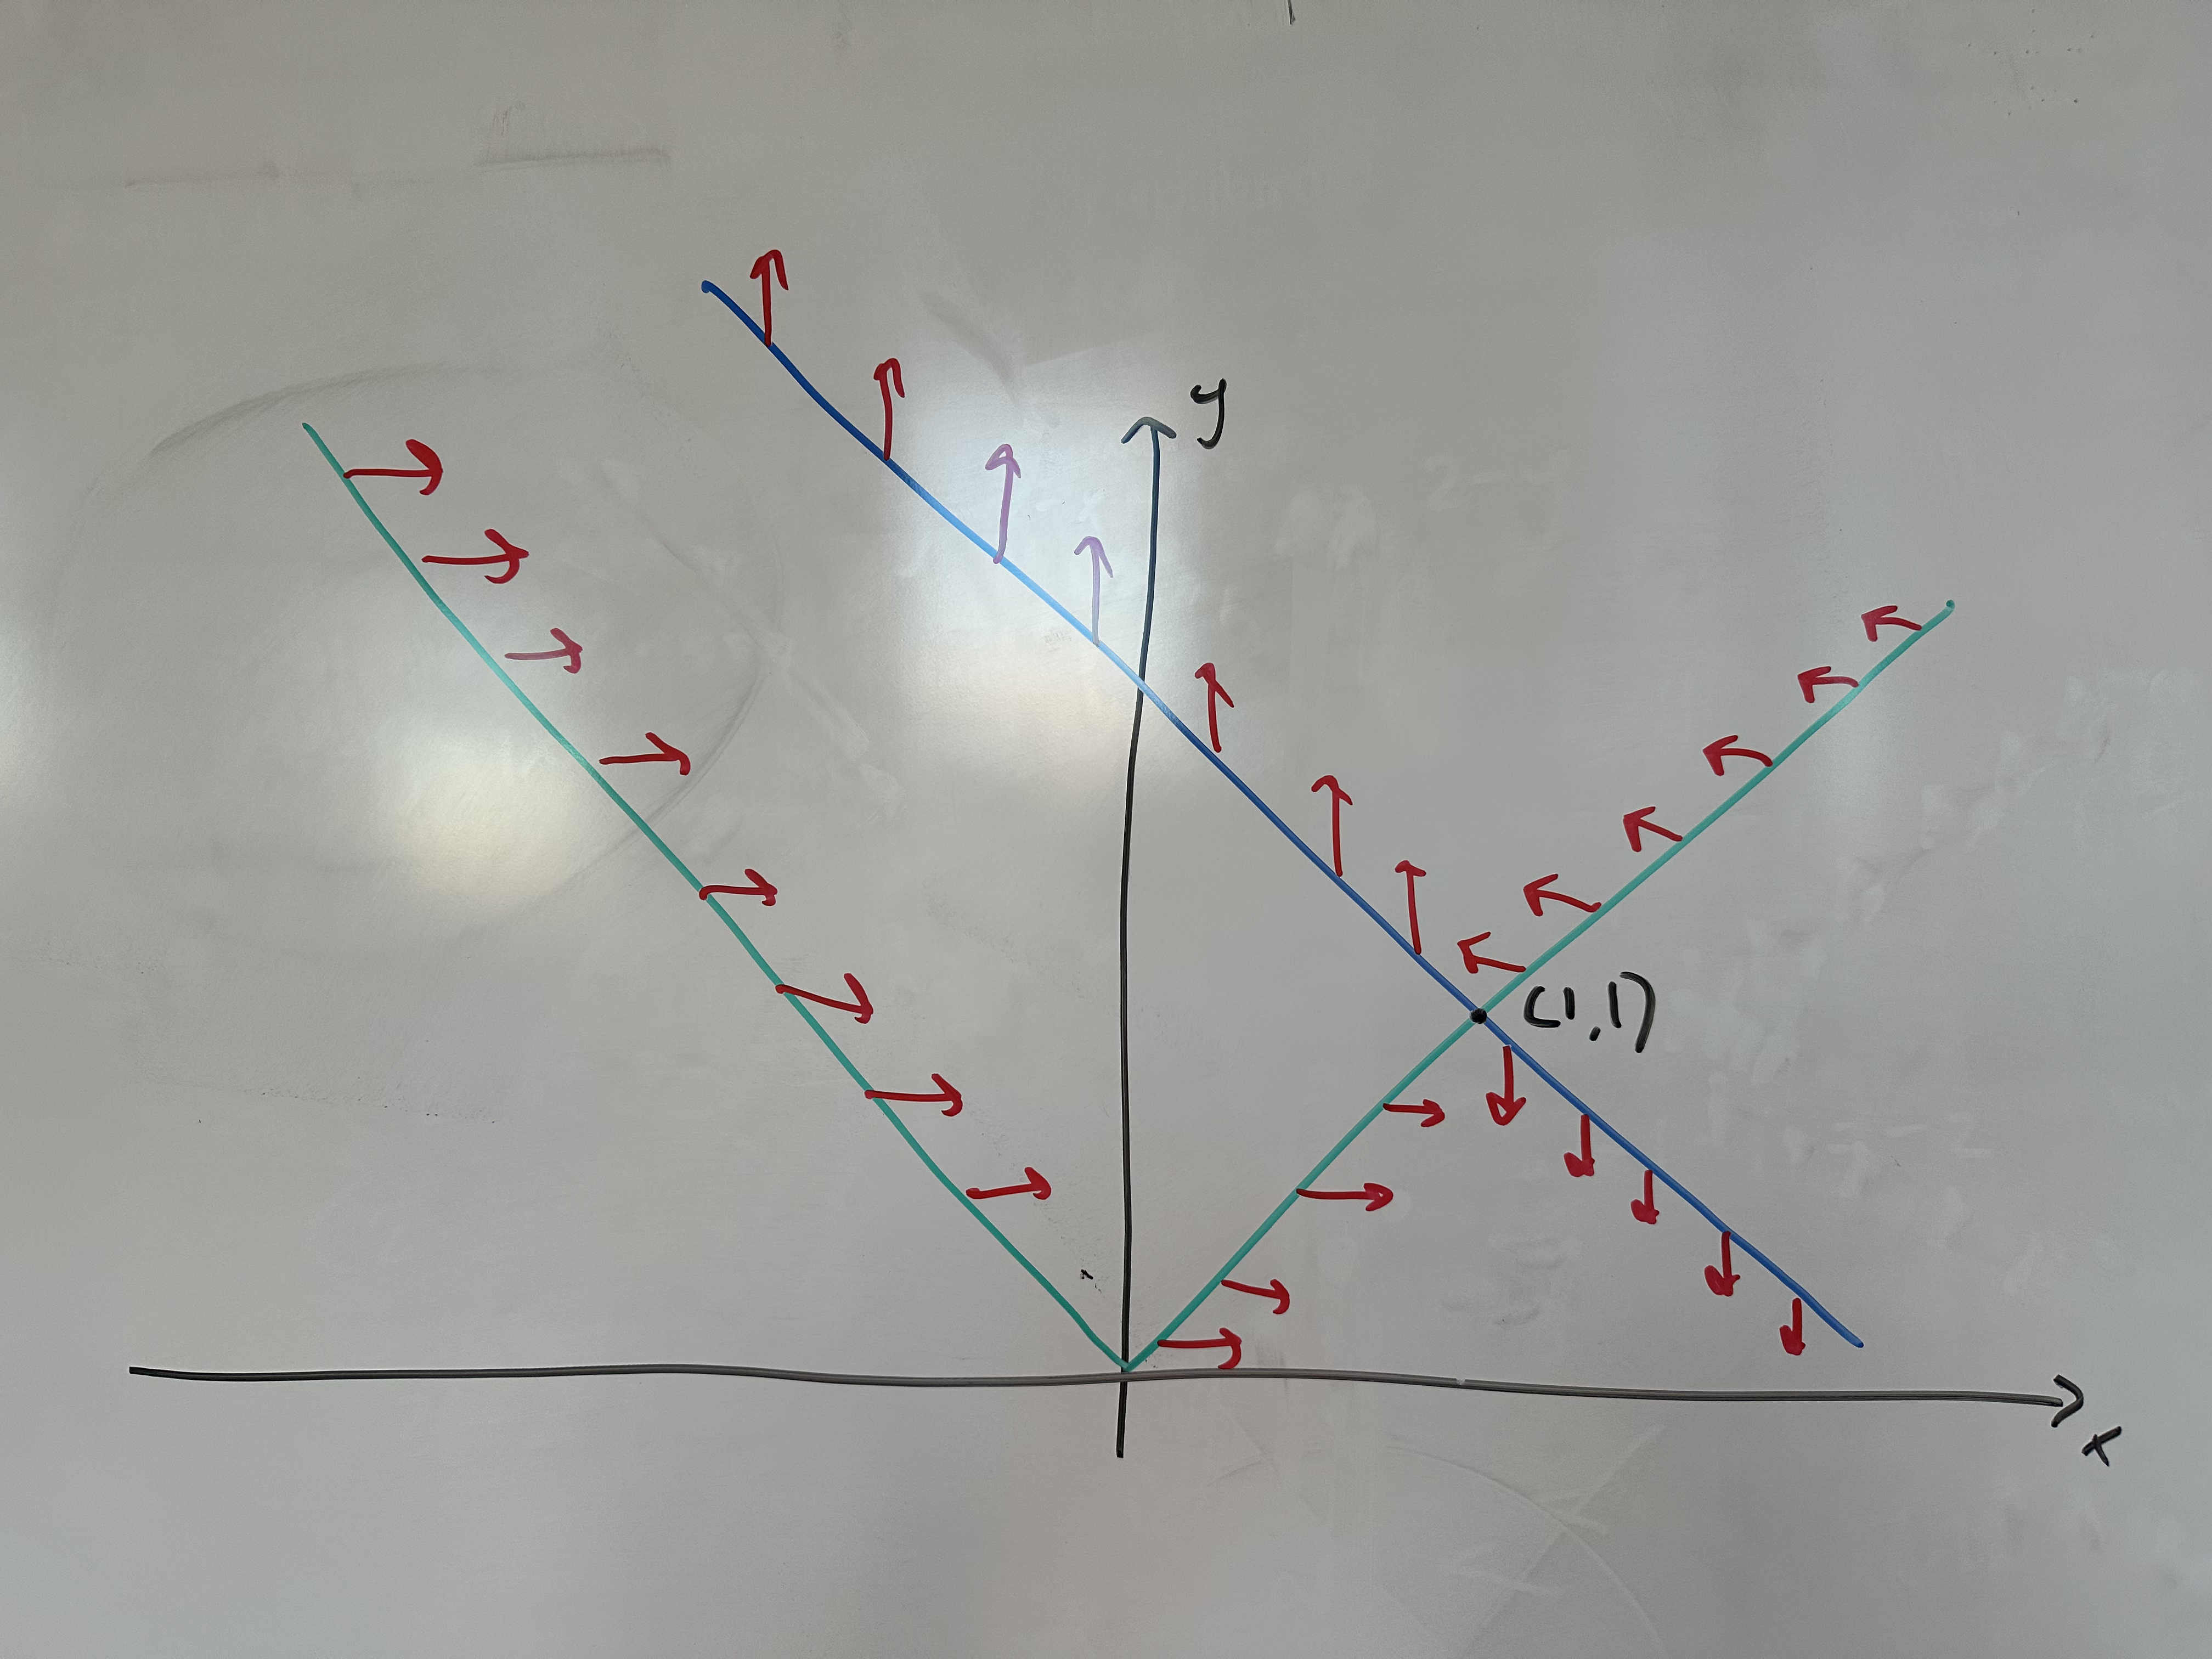
\includegraphics[scale=0.05]{IMG_3007.png}
	\centering
\end{figure}

A solution starting at $(-1,1)$ will be on the $y$-nullcline, so will move to the left and then begin drifting up. It should diverge towards $\infty$ along the $y$-direction, and its $x$ direction divergence will likely be positive, although it depends on the separatrix.

A solution starting at $(2,1)$ will have to either move downwards towards the $x$-nullcline, or upwards towards the $y$-nullcline. Evaluating $\frac{\mathrm{d}y}{\mathrm{d}t} $ at this point gives
\[
	\frac{\mathrm{d}y}{\mathrm{d}t} =1>0
.\]
Therefore, the solution will move upwards, and diverge towards positive $\infty$ in the $y$ direction. It should align with the same separatrix that bounds the previous point, but on the other side.

For the solution starting at $(2,2)$, notice that it starts on the $y$-nullcline, and will move left and diverge towards positive $\infty$ in the $y$ direction, once again along the same separatrix.
\section*{Section 5.2 Problem 5}
Setting $\frac{\mathrm{d}x}{\mathrm{d}t} =0$, we find either $x=0$ or
\[
	y=-\frac{1}{3}x+50
.\]
Setting $\frac{\mathrm{d}y}{\mathrm{d}t} =0$, we find either $y=0$ or
\[
	y=-2x+100
.\]
Setting them equal to each other, we have
\[
	-\frac{1}{3}x+50=-2x+100\implies x=30
.\]
It follows that $y=40$.

Consider the vector field along $x$-nullclines. Setting $x=0$, we have
\[
	\frac{\mathrm{d}y}{\mathrm{d}t} =y(-y+100)
.\]
Notice that this is greater than $0$ for $y<100$, and less than $0$ otherwise. There is then a sink at $(0,100)$. Now let $x=3y-150$. We have
\[
	\frac{\mathrm{d}y}{\mathrm{d}t} =y\left( -2\left( 3y-150 \right) -y+100 \right) =y\left( -5y+200 \right) 
.\]
Notice that this quantity is greater than $0$ for $y<40$, and less than 0 otherwise. Finally, consider the $y$-nullclines. For $y=0$, we have
\[
	\frac{\mathrm{d}x}{\mathrm{d}t} =x(-x+150)
.\]
This is positive for $x<150$, and negative otherwise. Now let $y=-2x+100$. We have
\[
	\frac{\mathrm{d}x}{\mathrm{d}t} =x(-x-3\left( -2x+100 \right) +150)=x(5x-150)
.\]
This will be negative for $x<30$, and positive otherwise. We can now give the phase plane.
\begin{figure}[ht]
	
\includegraphics[scale=0.25]{../figures/image0.jpg}
	\centering
\end{figure}
\newpage
All solutions will eventually collapse to one of the two sinks along the axes.
\section*{Section 5.2 Problem 18}
We end up with the $a$-nullcline being the line
\[
	a\left( \frac{1}{3}a+\frac{1}{2}b \right) =2
.\]
The $b$-nullclines are $a,b=0$ and $ab=3$. I plotted these equations with computer software. Start by considering the $b$-nullclines. For $a=0$, we have $\frac{\mathrm{d}a}{\mathrm{d}t} =2$. For $b=0$, we have
\[
	\frac{\mathrm{d}a}{\mathrm{d}t} =2-\frac{a^2}{3}
.\]
We end up with $a=\sqrt{6} $ being an equilibrium point, with $\frac{\mathrm{d}a}{\mathrm{d}t} >0$ below it and $<0$ above it. Now suppose $ab=3$. We have
\[
	\frac{\mathrm{d}a}{\mathrm{d}t} =2-\frac{3}{2}-\frac{a^2}{3}=\frac{1}{2}-\frac{a^2}{3}
.\]
We end up with $a=\sqrt{3 /2} $ as an equilibrium point, and $\frac{\mathrm{d}a}{\mathrm{d}t} >0$ for $a$ less than this, and less than 0 otherwise.

Now consider the $a$-nullcline. We can solve for $ab$ of the form
 \[
	ab=4-\frac{2}{3}a^2
.\]
Plugging this in yields
\[
	\frac{\mathrm{d}b}{\mathrm{d}t} =\frac{3}{2}-\frac{4-\frac{2}{3}a^2}{2}
.\]
We can try and solve for the equilibrium point. We have
\[
	3=4-\frac{2}{3}a^2\implies a=\sqrt{\frac{3}{2}}
.\]
We then know for $a<\sqrt{3 /2} $, $\frac{\mathrm{d}b}{\mathrm{d}t} >0$, and otherwise it will be less than $0$. Consider the following figure.
\begin{figure}[ht]
	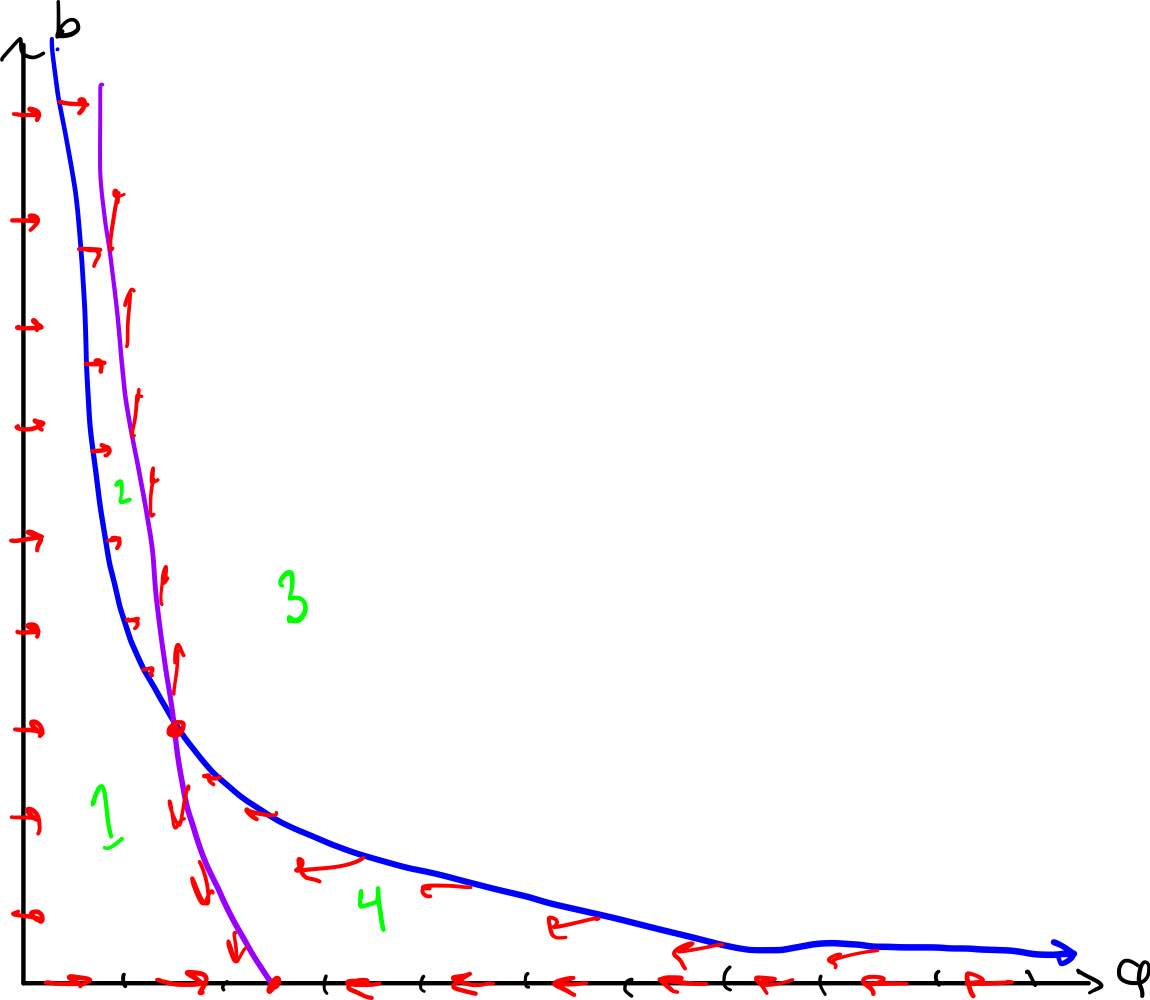
\includegraphics[scale=0.25]{../figures/image1.jpg}
	\centering
\end{figure}
Region 1 has increasing $a$ and decreasing $b$. Region 2 has increasing $a$ and $b$. Region 3 has decreasing $a$ and increasing $b$. Region 4 has decreasing $a$ and $b$.

Solutions can never leave region 4, and will collapse towards the equilibrium point. Solutions also appear to not be able to leave region 2, since $\frac{\mathrm{d}a}{\mathrm{d}t} $ will only approach $0$ as $t\to \infty$, so solutions will approach the $b$-nullcline, but never cross it.Solutinos can leave all other regions, but most solutions in region 3 appear to stay in region 3 and diverge to infinity.

\begin{mdframed}[linewidth=1pt]
	\begin{center}\bfseries
		PDE for Supplimental Problems
	\end{center}
	\[
		\frac{\partial u}{\partial t} =\frac{\partial ^2u}{\partial x^2} ,\qquad 0<x<\pi ,\;\;\; t>0
	,\]
	\[
		u(x,0)=u_0,\qquad \frac{\partial u}{\partial x} (0,t)=\frac{\partial u}{\partial x} (\pi ,t)=0
	.\]
\end{mdframed}
	Remember that
	\[
		\Phi_u(x,t)\propto \frac{\partial u}{\partial x} 
	,\]
	which is why we represent the boundary conditions in this way.
\section*{Supplimental 1}
Suppose $u(x,t)=e^{\lambda t}\phi (x)$ is a solution to the given problem. We have
\[
	\frac{\partial u}{\partial t} =\lambda e^{\lambda t}\phi (x)
\]
and
\[
	\frac{\partial ^2u}{\partial x^2} = e^{\lambda t}\frac{\partial ^2\phi }{\partial x^2}
.\]
Since $\phi $ is a function only in $x$,
\[
	\frac{\partial ^2\phi }{\partial x^2} =\frac{\mathrm{d}^2\phi }{\mathrm{d}x^2} 
.\]
We then have
\[
	e^{\lambda t}\frac{\mathrm{d}  ^2\phi }{\mathrm{d}  x^2} =\lambda e^{\lambda t}\phi (x)
.\]
Since $e^{\lambda t}\neq 0$ for all $t\in\mathbb{R}$, we cancel the exponentials and have
\begin{equation}\label{eq:1}
	\frac{\mathrm{d}^2\phi }{\mathrm{d}x^2} =\lambda \phi (x)
.\end{equation}
Therefore, if $u(x,t)=e^{\lambda t}\phi (x)$ solves the given problem, then $\phi $ satisfies (\ref{eq:1}).
\section*{Supplimental 2}
I'm going to write $\phi_n$ and $\phi _m$ instead of $\phi _n(x)$ and $\phi _m(x)$, because it got fairly messy and that felt cleaner. Let $\phi_n(x),\lambda_n$ and $\phi_m(x),\lambda_m$ solve the given PDE. We have
\begin{align*}
	\lambda_n \left<\phi_n,\phi_m \right> &=\lambda_n\int_{0}^{\pi } \phi _n\phi _m  \,\mathrm{d} x\\
						    &=\int_{0}^{n} \lambda _n\phi _n\phi _m \,\mathrm{d} x
.\end{align*}
Since $\phi _n,\lambda _n$ solve the PDE, they must satisfy (\ref{eq:1}). It follows by the method of integration by parts that
\begin{align*}
	\int_{0}^{n} \lambda _n\phi _n\phi _m \,\mathrm{d} x&=\int_{0}^{\pi } \frac{\mathrm{d}  ^2\phi _n}{\mathrm{d}  x^2} \phi _m \,\mathrm{d} x\\
								  &=\left[ \frac{\mathrm{d}\phi _n}{\mathrm{d}x} \phi _m \right]_0^\pi -\int_{0}^{\pi } \frac{\mathrm{d}\phi _n}{\mathrm{d}x} \frac{\mathrm{d}\phi _m}{\mathrm{d}x}  \,\mathrm{d} x\\
								  &=\left[ \frac{\mathrm{d}\phi _n}{\mathrm{d}x} \phi _m \right]_0^\pi -\left[ \phi_n \frac{\mathrm{d}\phi _m}{\mathrm{d}x}  \right]_0^\pi +\int_{0}^{\pi } \phi_n\frac{\mathrm{d}^2\phi _m}{\mathrm{d}x^2}  \,\mathrm{d} x
.\end{align*}
Consider the boundary conditions. We have
\[
	\frac{\partial u}{\partial x} (0,t)=\frac{\partial u}{\partial x} (\pi ,t)=0
.\]
Notice that
\[
	\frac{\partial u}{\partial x} =e^{\lambda t}\frac{\partial \phi }{\partial x} =e^{\lambda t}\frac{\mathrm{d}\phi }{\mathrm{d}x} 
.\]
Since $e^{\lambda t}\neq 0$ for all $t$, we must have
\[
	\frac{\mathrm{d}\phi }{\mathrm{d}x} (0)=\frac{\mathrm{d}\phi }{\mathrm{d}x} (\pi )=0
\]
for all $\phi $ solving the PDE. Using this fact, we have
\begin{align*}
	\left[ \frac{\mathrm{d}\phi _n}{\mathrm{d}x} \phi _m \right]_0^\pi -\left[ \phi_n \frac{\mathrm{d}\phi _m}{\mathrm{d}x}  \right]_0^\pi +\int_{0}^{\pi } \phi_n\frac{\mathrm{d}^2\phi _m}{\mathrm{d}x^2}  \,\mathrm{d} x&=\int_{0}^{\pi } \phi _n \frac{\mathrm{d}^2\phi _m}{\mathrm{d}x^2}  \,\mathrm{d} x\\
																												  &=\int_{0}^{\pi } \phi_n \lambda _m \phi _m \,\mathrm{d} x\\
																												  &=\lambda_m \int_{0}^{\pi } \phi _n\phi _m \,\mathrm{d} x\\
																												  &=\lambda _m \left<\phi _n,\phi _m \right>	
.\end{align*}
Therefore,
\[
	\lambda_n \left<\phi _n,\phi _m \right> = \lambda_m \left<\phi _n,\phi _m \right>
.\]
Notice that if $\left<\phi _n,\phi _m \right>\neq 0$, then $\lambda _n=\lambda _m$, a contradiction. Therefore, $\left<\phi _n,\phi _m \right> = 0$.
\section*{Supplimental 3}
Suppose
\[
	\phi (x)=A\cos (\omega x)+B\sin (\omega x)
,\]
where $\lambda =-\omega ^2$. We have
\[
	\frac{\mathrm{d}\phi }{\mathrm{d}x} =-A\sin (\omega x)+B\cos (\omega x)
.\]
Using our boundary conditions, we know
\[
	-A\sin (0)+B\cos (0)=B=0
.\]
Therefore, $B=0$. Additionally,
\[
	-A\sin (\omega \pi )=0
.\]
This occurs if and only if $\omega \pi =n\pi $ for some $n\in\mathbb{Z}$. Therefore, we have
\[
	\phi_n (x)=A_n\cos (nx)
.\]
Moreover, $\lambda_n=-n^2$. Notice that for the case $n=0$, we have the constant solution $\phi_0(x)=A_n\cos (0)=0$.
\section*{Supplimental 4}
Let
\[
	u(x,t)=\sum_{n=0}^{\infty} A_n e^{-n^2t}\cos  (nx)
.\]
Let $t=0$ to consider our initial conditions. We will determine the coefficients $A_n$ subject to the initial condition. We have
\[
	u_0(x)=\sum_{n=0}^{\infty} A_n\cos  (nx)
.\]
Multiplying both sides by $\cos  (kx)$ for some fixed $k\in\mathbb{N}$, we have
\begin{align*}
	&\qquad\;\;\; \cos  (kx)u_0\left(x \right) =\cos (kx)\sum_{n=0}^{\infty} A_n \cos  (nx)\\
	&\implies \cos  (kx)u_0(x)=\sum_{n=0}^{\infty} A_n\cos  (kx)\cos  (nx)\\
	&\implies \int_{0}^{\pi } \cos  (kx)u_0(x) \,\mathrm{d} x=\int_{0}^{\pi } \sum_{n=0}^{\infty} A_n \cos  (kx)\cos  (nx) \,\mathrm{d} x\\
	&\qquad\qquad\qquad\qquad\qquad\quad\;=\sum_{n=0}^{\infty} \int_{0}^{\pi } A_n \cos  (kx)\cos  (nx) \,\mathrm{d} x\\
	&\qquad\qquad\qquad\qquad\qquad\quad\;=\sum_{n=0}^{\infty} \left<A_n\phi_n,\phi_k \right>\\
	&\qquad\qquad\qquad\qquad\qquad\quad\;=\sum_{n=0}^{\infty} A_n\left<\phi_n,\phi_k \right> \\
	&\qquad\qquad\qquad\qquad\qquad\quad\;=A_k\left\lVert \phi_k \right\rVert^2
.\end{align*}
We then have
\begin{align*}
	A_k&=\frac{\int_{0}^{\pi } \sin (kx)u_0(x) \,\mathrm{d} x}{\int_{0}^{\pi } \cos^2(kx) \,\mathrm{d} x}\\
	   &=\frac{\int_{0}^{\pi } \cos (kx)u_0(x) \,\mathrm{d} x}{\frac{1}{2}\int_{0}^{\pi } 1+\cos (2kx) \,\mathrm{d} x}\\
	   &=\frac{\int_{0}^{\pi } \cos (kx)u_0(x) \,\mathrm{d} x}{\frac{1}{2}\left[ x+\frac{1}{2k}\sin(x) \right]_0^\pi }\\
	   &=\frac{\int_{0}^{\pi } \cos (kx)u_0(x) \,\mathrm{d} x}{\frac{\pi }{2}}\\
	   &=\frac{2}{\pi }\int_{0}^{\pi } \cos (kx)u_0 \,\mathrm{d} x\\
	   &=\frac{2}{\pi }\left<\phi_k,u_0 \right>
.\end{align*}
The above statements follow for the case $n\neq 0$. For $n=0$, we have $\phi_0(x)=\cos 0=1$. It follows that
\[
	\int_{0}^{\pi } u_0(x)1 \,\mathrm{d} x=\sum_{n=0}^{\infty} \int_{0}^{\pi } A_n\cos (nx)1 \,\mathrm{d} x=\int_{0}^{\pi } A_0 \,\mathrm{d} x=\pi A_0
.\]
Therefore,
\[
	A_0=\frac{1}{\pi }\int_{0}^{\pi } u_0 \,\mathrm{d} x=\frac{1}{\pi }\left<u_0,1 \right>
.\]

Therefore,
\[
	u(x,t)=\frac{1}{\pi }\left<u_0,1 \right>+\frac{2}{\pi }\sum_{n=1}^{\infty} e^{-n^2t}\left<\phi_n,u_0 \right> \cos(nx)
.\]
\end{document}
